% LaTeX Template for Project Report, Version 2.0
% (Abstracted from a Major Project Report at CSED, NIT Calicut but can be
% modified easily to use for other reports also.)
%
% Released under Creative Commons Attribution license (CC-BY)
% Info: http://creativecommons.org/licenses/by/3.0/
%
% Created by: Kartik Singhal
% BTech CSE Batch of 2009-13
% NIT Calicut
% Contact Info: kartiksinghal@gmail.com
%
% It is advisable to learn the basics of LaTeX before using this template.
% A good resource to start with is http://en.wikibooks.org/wiki/LaTeX/
%
% All template fields are marked with a pair of angular brackets e.g. <title here>
% except for the ones defining citation names in ref.tex.
%
% Empty space after chapter/section/subsection titles can be used to insert text.
%
% Just compile this file using pdflatex after making all required changes.

\documentclass[12pt,a4paper]{article}
\usepackage{amssymb}
\usepackage{ctex}
%\usepackage{graphicx}
\usepackage{caption}
\usepackage{algorithm}
\usepackage{algpseudocode}

\begin{document}

\begin{center}
{\LARGE ICTCP: Incast Congestion Control for TCP in Data Center Networks Final Report
}
\end{center}
\noindent{\textbf{Group member:}}

Anni Du                 Student ID: 110947646\\
Tianyao Luo         	Student ID: 110974260\\
Yishuo Wang 	      	Student ID: 108533945\\

\noindent{\textbf{Abstract}}

\noindent{Our} topic is ICTCP: Incast Congestion Control for TCP in Data Center Networks. In data center networks, TCP incast congestion happens on high-bandwidth and low latency networks, when multiple synchronized servers send data to a same receiver in parallel. For many popular application, this issue is in common. Incast congestion happens when the buffer of Ethernet switch buffer is overflowed by multiple TCP connections, which causes package loss and TCP timeout. If incast congestion happens, the throughput and bandwidth utilization ratio will be very low. The paper introduce a new way named Incast Congestion Control for TCP (ICTCP) to figure out the problem. The scheme works on the receiver side. Easily to see, the ICTCP adjusts TCP receive window in advance before the packet drops occur. For the result, the paper achieve almost zero timeout and high goodput for TCP incast. Our group is not as perfect as the paper, but we can decrease the loss rate and increase the goodput successfully.[1]

\section{Introduction}

\noindent{We} know the TCP(Transport Control protocol) is super popular in the Network area as a transport layer protocol. However, many facts show us that it will have high loss rate or high packets loss when many servers send to one server parallel at the same time, especially on high-bandwidth, low latency networks. To figure out the problem, paper build ICTCP.

\noindent{To} achieve the paper, our group divides the project into five steps. First, because of our actual condition, we can not build an environment as perfect as the paper, so we decide to use NS-3 to build the environment, which is recommended by professor. Second, after setting up the environment successfully, we will simulate the problem, which is many-to-one traffic. Third, by reading the paper, we will follow the paper to achieve ICTCP. Fourth, we will try to do some improve on the ICTCP case to see if we can let the performance better. Fifth, in all the steps above, we need to record the data, so in this step, we will compare these data to analyze the problem and our work.

\noindent{We} know most of people use changing congestion window size to decrease the loss rate, but the paper is not. They focus on the receive side, which means we will focus on changing the receive window.

\noindent{The} reason not changing the congestion window is that, the smaller change we make to the existing system, the better. Therefore, a solution that modifies TCP receiver only is preferred than solutions that require switches and routers support (such as ECN) and modifications at both TCP sender and receiver sides.

\noindent{Finally}, we achieve decreasing the loss rate in many-to-one traffic. The paper use 48 server totally, which means paper will use at most 47 servers send to one server at the same time. Because of our actual situation, we can not hold 48 servers. We decide to use 16 servers to simulate the problem, so we will have at most 15 servers to send one server parallel.

\section{Environment setup}
\noindent{Because} of the recommendation by the professor, we decide to use NS-3 to simulate the problem. To set up NS-3 successfully, we will use VirtualBox to implement a virtual machine, which we decide to use Fedora.

\noindent{After} we install Fedora successfully, we need to install some library to support the NS-3, the command is following[2].


\begin{verbatim}
dnf install gcc gcc-c++ python
dnf install gcc gcc-c++ python python-devel
dnf install mercurial
dnf install bzr
dnf install gsl gsl-devel
dnf install gtk2 gtk2-devel
dnf install gdb valgrind
dnf install doxygen graphviz ImageMagick
dnf install python-sphinx dia texlive texlive-latex
dnf install flex bison
dnf install tcpdump
dnf install sqlite sqlite-devel
dnf install libxml2 libxml2-devel
dnf install uncrustify
dnf install openmpi openmpi-devel
dnf install boost-devel
dnf install redhat-rpm-config goocanvas-devel graphviz graphviz-devel python-setuptools python-kiwi pygoocanvas ipython
 easy_install pygraphviz
dnf install qt4-devel
dnf install cmake glibc-devel.i686 glibc-devel.x86_64
dnf install patch autoconf cvs
\end{verbatim}

\noindent{Then} we will download NS-3 using Mercurial. The command is following.	[2]

\begin{verbatim}
cd
mkdir repos
cd repos
hg clone http://code.nsnam.org/ns-3-allinone
\end{verbatim}

\noindent{In} the directory ``~/repos/ns-3-allinone'', We run[2]

\begin{verbatim}
./download.py -n ns-3-dev
\end{verbatim}

\noindent{Then} we can start to build NS-3. In the directory ``~/repos/ns-3-allinone'', We run[3]
\begin{verbatim}
./build.py � enable-examples �enable-tests
\end{verbatim}

\noindent{This} process will last about 20 mins to 30 mins. Then we run ``./test.py'', and this process will last about 40 mins to 60 mins. If all the case pass, which means we set up the environment successfully.

\section{Data center Topology}
\noindent{In} the paper, the author uses 48 servers and let at most 47 servers send to one server at the same time. Because of our condition, we decide to use 16 servers totally to simulate the problem.
\begin{figure}[h!]
\begin{center}
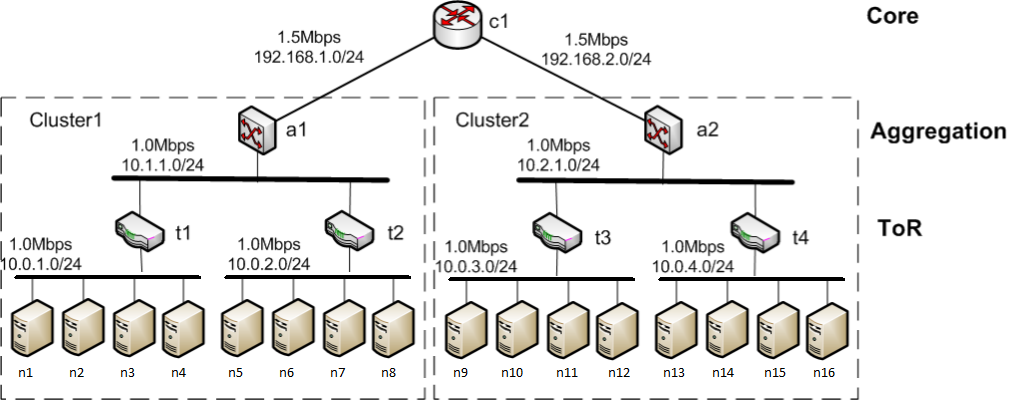
\includegraphics[width=\textwidth]{network.png}
\end{center}
\end{figure}

\section{Simulate TCP incast congestion control}


\noindent{For simulate the incast congestion control in data center. We simply send packets from the server 2-16 to server 1. To avoid other influence as much as possible, we use a fixed sending rate which equals 1 Mbps, the size of packets equals to 2000 bytes. In NS-3, we first build a topology like the section 3, then we let 1 server(n2) send to server 1,(n1) and let 2 servers(n2, n3) send to server 1(n1) parallel, etc. Each time increase one sending server, until we use 15 servers(n2 � n16) to send packets to server 1(n1) parallel. Therefore, we have fifteen group of data in total. We outputted fifteen ``.pcap'' files for each of these group of data correspondingly. By parsing these ``.pcap'' files, we get the loss rate and the goodput when the many-to-one traffic problem happens. To calculate the goodput, we use the following equation.}
\[
goodput = \frac{the\ total\ bytes\ that\ receiver\ get\ succfessfully}{the\ total\ time}
\]

\noindent{Then} we change the unit to Mbps. And the following the goodput graph in normal TCP. We can see that with the increasing of the number of sending server, the goodput will change, which is caused by the packet drops.

\noindent{To calculate the loss rate, at first we use the retransmission to calculate.}
\[
loss\ rate = \frac{the\ number\ of\ the\ retransmission\ packets}{total\ number\ of\ packets\ send}
\]
\noindent{However, the graph we get is not that similar with the graph paper shows us. Following is the graph. }
\begin{figure}[h!]
\begin{center}
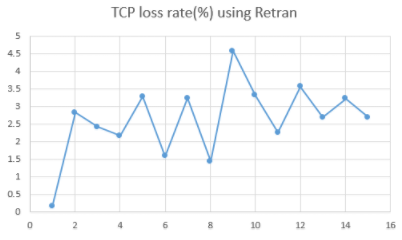
\includegraphics[width=0.7\textwidth]{4-1.jpg}
\end{center}
\end{figure}

\noindent{Then we decide to use another way to calculate the loss rate. The equation is}

\[
loss\ rate = \frac{total\ number\ of\ packets\ send - the\ number\ of\ packets\ receiver\ get}{total\ number\ of\ packets\ send}
\]

\noindent{After collecting data to draw the graph, we get a new loss rate graph(above).}

\begin{figure}[h!]
\begin{center}
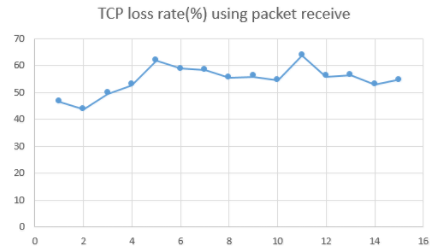
\includegraphics[width=0.7\textwidth]{4-2.jpg}
\end{center}
\end{figure}

\noindent{From the loss rate graph, we can see even though not that obvious, but our data loss rate does increases with the sending server number increasing. Then, our goal is to achieve the ICTCP to decrease the loss rate.}

\section{Doing Throughput-based window control  on same topology}

\noindent{After read the paper carefully, we fully understood the algorithm of ICTCP. }

\noindent{\textbf{Thoughts:}}ICTCP uses difference ratio of measured and expected throughput as an indicator to change the receive window size.

\noindent{\textbf{Key factor:}}The algorithm to compute the difference ratio is as follows.
1. Compute measured throughput $b_i^m$ using formula(1)
\[
b_{i,new}^m = \max(b_i^s, \beta * b_{i,old}^m + (1-\beta) * b_i^s)\ \ \ \ (1)
\]

where $b_i^s$ is the sample current throughput, and $\beta$ is the parameter that can be changed. In our experiment we set $\beta = 0.5$.\\

2.Compute expected throughput $b_i^e$ using formula(2)
\[
b_i^e = \max(b_i^m, rwnd_i / RTT_i)\ \ \ \ (2)
\]
where $b_i^m$ is the current measured throughput and $rwnd_i$, $RTT_i$ represent current receive window size and current RTT, respectively.\\

3. Compute the difference ratio of measured and expected $d_i^b$ throughput using formula(3)
\[
d_i^b = (b_i^e - b_i^m) / b_i^e\ \ \ \ (3)
\]


\noindent{\textbf{Updating rule:}}ICTCP introduces two thresholds $\gamma_1$ and $\gamma_2$ to control when we will change the window size. We list three updating situations below.

\begin{enumerate}
\item $d_i^b \leq \gamma_1$ or $d_i^b \leq MSS_i/rwnd_i$ means there are enough buffer in receiver side, so we increase the receive window size.
\item $d_i^b \geq \gamma_2$ and these situations last for three transactions, which means the buffer of receiver side is about to overflow. In other words, there is a high probability of loss. Therefore, the receive window size has to decrease.
\item otherwise, we didn�t do anything to the receive window size.
\end{enumerate}

\noindent{\textbf{Updating detail:}}The way to change the receive size is similar to the way to change the congestion window size.

\begin{enumerate}
\item The minimum rwnd is 2 MSS.
\item In condition of updating rule 2, we decrease the rwnd by 1 MSS while we maintain that the rwnd is no less than the minimum rwnd size.

\item in condition of updating rule 1, we increase the rwnd follow the ``slow start'' process and ``congestion avoidance'' process.
\item using available bandwidth $BW_a$ to decide when to use ``slow start'' and when to use ``congestion avoidance''. $BW_a$ is computed using formula(4).
\end{enumerate}
\[
BW_a = \max(0, \alpha * C - BW_T)\ \ \ \ (4)
\]


where C is the link capacity of the interface on receiver server, $BW_T$ is the total incoming traffic observed on that interface and $\alpha$ is the parameter that can be changed. In our experiment , we set $\alpha=0.9$.

\noindent{\textbf{5.1 Introduce ICTCP updating rules to congestion window size:}}

\noindent{Our first customized TCP is applying ICTCP updating rules to control congestion window size. We call it ICTCP-C.}

\noindent{The algorithm of ICTCP-C is defined as following:}

\noindent{\textbf{function $Increase_Window()$}}

\begin{enumerate}
\item $d_i^b$ = $Compute_Ratio$
\item if  $d_i^b \leq \gamma_1$ or  $d_i^b\leq MSS_i/rwnd_i$
\item if $rwnd_i \leq SSH$, run new Reno�s Slow Start phase.
\item else run new Reno�s Congestion Avoidance phase.
\item else  do nothing.
\end{enumerate}

\noindent{\textbf{function $Set_Shh_Threshold()$}}

\begin{enumerate}
\item if  $d_i^b \geq \gamma_2$ and $m\_count\geq 2$, return $rwnd_i - MSS_i$
\item else if $d_i^b \geq \gamma_2$ , $m\_count = m\_count + 1$
\item else return $cwnd_i$

\end{enumerate}



\noindent{\textbf{Thoughts:}}
\noindent{\textbf{Thoughts:}}




\noindent{The algorithm of ICTCP-C is defined as following:}

\noindent{}

\noindent{}

\noindent{}

\noindent{}

\noindent{}

\noindent{}

\noindent{}

\noindent{}


\noindent{}

\begin{figure}[h!]
\begin{center}
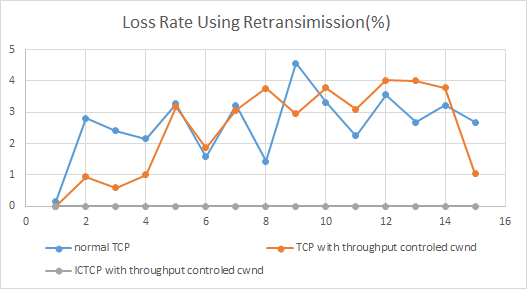
\includegraphics[width=0.8\textwidth]{1.jpg}
\end{center}
\end{figure}



\end{document}
